% Chapter 7

\chapter{Validación del desarrollo} \label{capitulo6}
El flujo de validación de las historias de usuario fue un proceso sistemático, consistente y controlado por parte de los desarrolladores y de los expertos en educación encargados de validar el software desarrollado. Las pruebas y otras validaciones abarcan las siguientes dimensiones:
\begin{itemize}
	\item Entradas, salidas y funciones del módulo curricular.
	\item Todos los requisitos no funcionales con sus respectivas pruebas. Como la utilización de tecnologías como Java, MySQL, Bootstrap, entre otras.
	\item Pruebas de rendimiento, fiabilidad, y tiempos de respuesta.
	\item Pruebas por parte de expertos de dominio.
	\item Verificación en diferentes clientes con diversos navegadores y sistemas operativos.
	\item Límites de intervalos, valores por defecto y valores específicos que el módulo acepta.
	\item Criterios de aceptación, especificaciones de requerimientos, funcionales y no funcionales expresados en las historias de usuario y otros documentos del proyecto.
\end{itemize}

Cabe resaltar que la documentación de los casos de prueba en Scrum no involucra necesariamente una secuencia paso a paso a ser utilizada en las pruebas y otros controles de calidad. Al mismo tiempo, los usuarios que validan las historias (expertos en educación en el marco de este proyecto), tienen amplia libertad para aceptar o rechazar las historias de usuarios entregadas por el equipo de desarrollo. 

Así también, los expertos de dominio tienen la potestad de pedir cambios a partir de la experiencia de utilización de las herramientas desarrolladas. Todos estos preceptos fueron observados en la realización de este trabajo.

En la figura \ref{workflow} se puede apreciar el ciclo de vida de las historias de usuario, donde una vez que es creada pasa al estado de \enquote{TODO}, que quiere decir que está pendiente a ser desarrollada. Una vez que un miembro del equipo de desarrollo comienza una historia o tarea pasa al estado de \enquote{IN PROGRESS} y cuando termina pasa al estado de \enquote{UNDER REVIEW}. 

En dicho estado se revisa la funcionalidad mediante validaciones de parte de los miembros del equipo de desarrollo y de parte del equipo de expertos en dominios de didáctica en universidades norteamericanas incluyendo a un PhD en educación, donde se deben cumplir los criterios de aceptación para que pase al estado de \enquote{CLOSED} que quiere decir que se terminó y que la historia fué aprobada.  

En caso de que la historia no consiga cumplir los criterios de aceptación correspondientes durante la validación se considera que la historia no está terminada y que debe pasar al estado de \enquote{REOPEN}, en este estado se puede pasar ya sea desde el estado \enquote{UNDER REVIEW} o si ya está en el estado \enquote{CLOSED}.

Cualquier otro problema o error de código que tenga la nueva funcionalidad se debe crear un ticket de error o bug especificando como reproducir el problema y el comportamiento esperado. En caso de no poder reproducir este comportamiento se pide más información al respecto o pasa al estado de \enquote{CLOSED} en caso de que el comportamiento ya no se pueda reproducir.

\begin{figure}[]
\centering
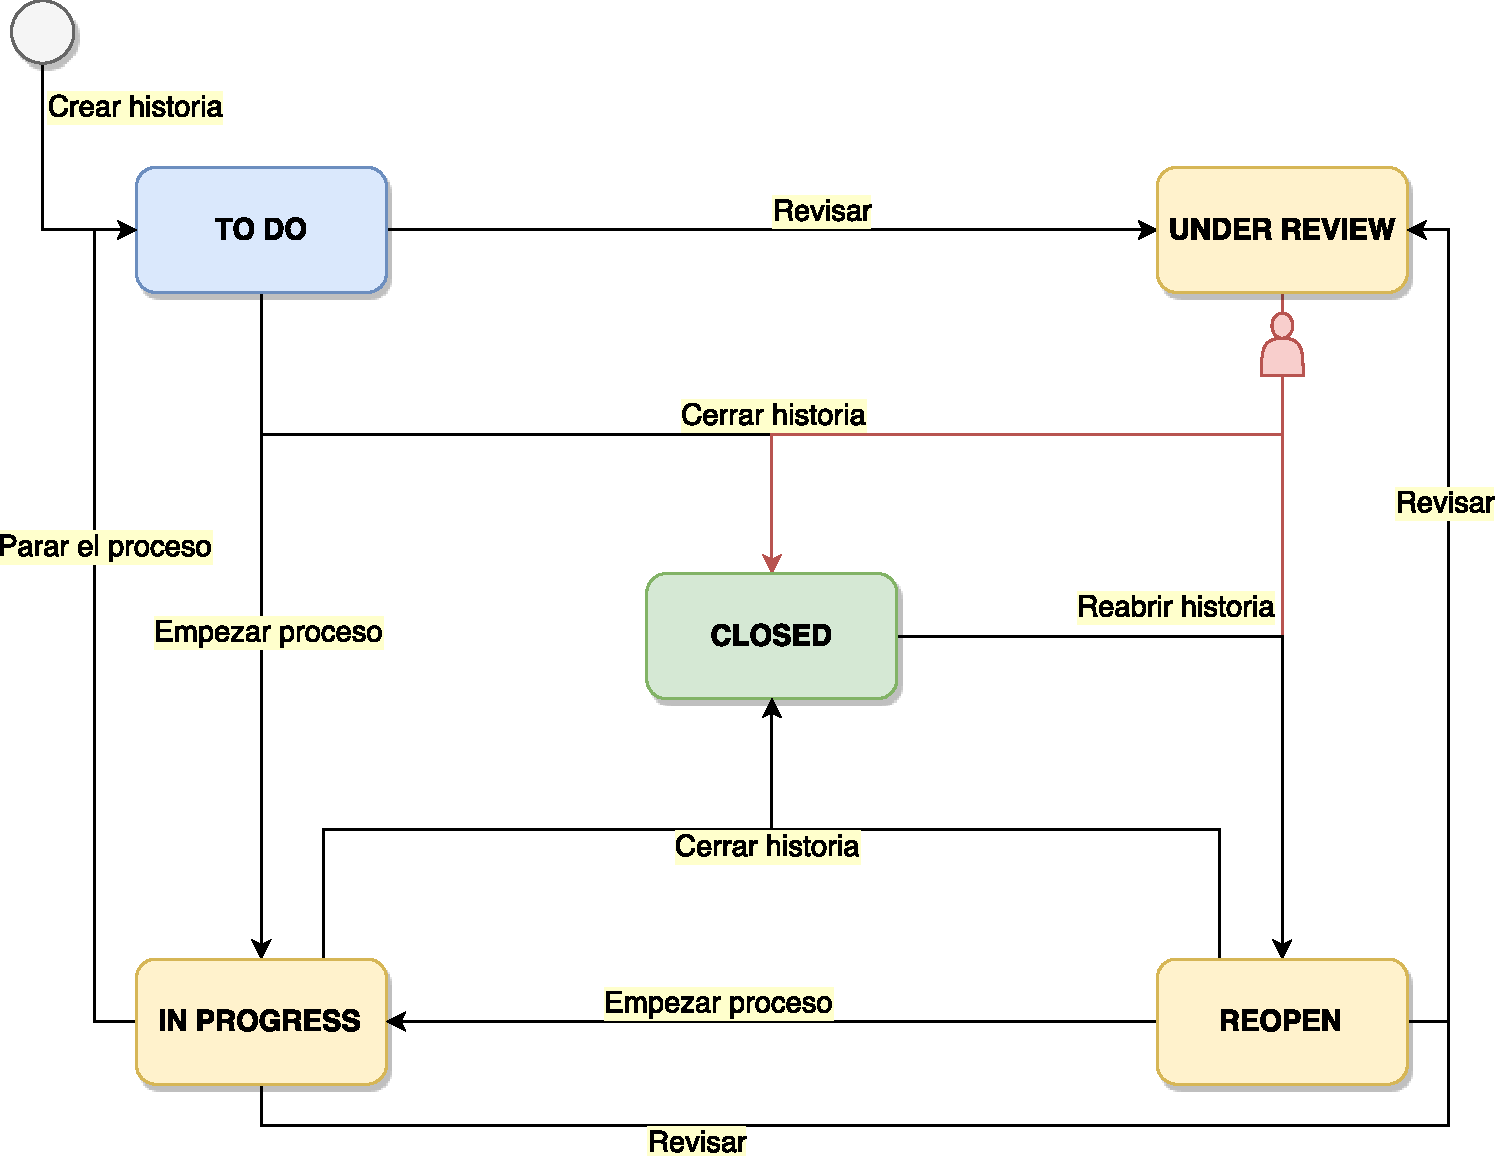
\includegraphics[scale=0.4]{Figuras/workflow}
\caption{Flujo de desarrollo de historias de usuario.}
  \label{workflow}
\end{figure}

\section{Revisión por pares}
Revisión por pares significa que los miembros del equipo de desarrollo revisa el código del otro miembro.

El equipo de desarrollo puede realizar evaluaciones por pares durante el desarrollo. La forma en que están sentados puede facilitar este proceso ya que puede dirigirse a la persona que está a su lado y pedirle que revise su trabajo. El equipo de desarrollo también puede reservar tiempo durante el día específicamente para revisar el código. Los equipos autogestionarios deben decidir qué es lo que funciona mejor para su equipo ya sea al inicio de cada iteración o luego de cierto periodo de pruebas.

Por cada funcionalidad terminada y aún en estado \enquote{In Progress} se procede a crear un PR\footnote{de sus siglas en inglés, Pull Request, que es una petición que el propietario de una rama del repositorio hace al propietario del repositorio original para que incorpore los commits que están en la rama.} desde la página de \enquote{GitHub}. 

La plantilla de los PR del repositorio tienen los siguientes campos:
\begin{itemize}
	\item \textbf{Descripción:} se describen los cambios en detalle, ya sea una nueva funcionalidad para el módulo o el problema, causa y cómo se arreglo una falla.
	\item \textbf{Pasos de prueba:} se describe de manera detallada los pasos que se siguieron para probar la rama. Por ejemplo, se coloca el usuario con el rol y cuáles fue la interacción del mismo con la aplicación.
	\item \textbf{Tipo de cambio:} si es una nueva funcionalidad, falla o cambio urgente al sistema.
	\item \textbf{Aceptación de términos y condiciones:} afirmando que se siguió la guía de buenas prácticas de código y que se leyó el documento con las reglas internas de escritura de código. Además, afirmando que las pruebas automatizadas nuevas y existentes pasan.
\end{itemize}

Y deben seguir los siguientes requisitos:
\begin{itemize}
	\item La rama debe estar probada desde una de las instancias del equipo en AWS. En caso de que las pruebas pasan, el usuario que no trabajó en la rama y que se encarga de probar la misma debe aprobar el PR desde la interfaz de revisión de \enquote{GitHub}.
	\item Se deben cumplir los criterios de aceptación y no debe agregar fallas al proyecto. En caso de encontrar fallas se debe notificar al propietario de la rama mediante comentarios desde la interfaz.
	\item Por cada rama en PR se ejecutan las pruebas automatizadas de karma.
	\item Debe pasar las reglas de código estático de la herramienta \enquote{Sonarqube}.
\end{itemize}

En caso de que uno de estos requisitos no se cumplan, \enquote{GitHub} no permite a los usuarios hacer la integración de la rama en el repositorio.

\section{Pruebas automatizadas}
Consiste en la automatización de pruebas por medio de código ejecutable, que permite controlar la ejecución de pruebas y la comparación entre los resultados obtenidos y esperados. Las pruebas automatizadas permiten incluir pruebas repetitivas y necesarias dentro de un ciclo de desarrollo para optimizar tiempo utilizado en pruebas manuales\citep{crispin2009agile}.

A menudo, el equipo de desarrollo desarrolla el código durante el día y corren las pruebas automatizadas durante la noche para tener los resultados a la mañana. Por la mañana, el equipo del proyecto puede revisar el informe de errores que generó el programa de pruebas, informar sobre cualquier problema durante el informe diario de cada desarrollador y buscar corregir esos problemas inmediatamente durante el día.

Algunas de las pruebas utilizadas son:
\begin{itemize}
	\item \textbf{Pruebas de integración:} 264 pruebas automatizadas de karma escritas para el módulo curricular, en la cual debían pasar las que hay en el sistema con las nuevas que se agregan.
	\item \textbf{Pruebas de exploración:} con el fin de asegurar la funcionalidad y la estabilidad del producto haciendo pruebas manuales buscando un comportamiento semejante a lo que haría un usuario normal.
	\item \textbf{Análisis de código estático:} 1221 reglas de Java de \enquote{Sonarqube} donde se informa sobre código duplicado, estándares de codificación, potenciales errores, comentarios y diseño del software.
\end{itemize}

Esto permitió comprobar que la aplicación funciona sobre los motores de javascript que la van a ejecutar, lo que nos ayudó a detectar posibles problemas por incompatibilidades de javascript entre ellos.

Con karma para las pruebas de interfaz, se decidió también el uso de la herramienta \enquote{Sonarqube} para evaluar el código fuente que se escribe para el módulo curricular. Donde dicha plataforma utiliza diversas herramientas de análisis estático de código funte para obtener métricas que pueden ayudar a mejorar la calidad del código del programa. Como ya se comentó, uno de los requisitos para que la funcionalidad pueda ser agregada al repositorio es que el PR pase las reglas que la plataforma impone.

\section{Revisión por parte del equipo de validación}
Una vez finalizado el proceso de desarrollo y verificación de las historias de usuario, el equipo de validación se encarga de revisar la funcionalidad y verifica que cumple con los criterios de aceptación. El equipo de validación forma parte del ciclo de vida de cada historia de usuario y hace las verificaciones acorde se agreguen a su lista de trabajos pendientes.

Finalmente, el propietario del producto debe comprobar y verificar que la historia de usuario en cuestión cumple con la definición de \enquote{DONE}. Cuando una historia de usuario cumple la definición de \enquote{DONE}, el propietario del producto actualiza la tabla de tareas moviendo la historia de usuario de la columna \enquote{UNDER REVIEW} a la columna \enquote{DONE}.

Por lo general, una vez que el sprint termina, se hace una revisión de las funcionalidades agregadas mediante una reunión utilizando la herramienta \enquote{GoToMeeting}, la cual sirve para reuniones desde cualquier parte del mundo con la capacidad de interactuar y compartir pantallas. El equipo de desarrollo muestra las nuevas funcionalidades y como se acceden a las mismas para facilitar la validación de parte del equipo experto en didáctica. Todos los errores o cambios pequeños de las historias se arreglan luego de la reunión o en caso de que sea muy grande y tome más de un día en arreglarse se procede a la creación de tickets de fallas.

Una vez finalizada la reunión, el equipo de validación y el equipo de desarrollo se comunican a través de la plataforma \enquote{Slack}, donde la misma permite compartir cualquier tipo de archivos, pantallas, y mantener una conversación accediendo desde cualquier plataforma. En la misma plataforma el equipo de validación hace sus consultas y reporta los errores antes de que cree tickets de falla en la plataforma \enquote{JIRA}.